%
\begin{tikzpicture}[
    image/.style={inner sep=0, outer sep=0, node distance = 0 and 0},
    label/.style={anchor=north west, fill=white, font=\small, xshift=1mm, yshift=-1mm}
]

    \node[image, anchor=south west] (image1)
    {
        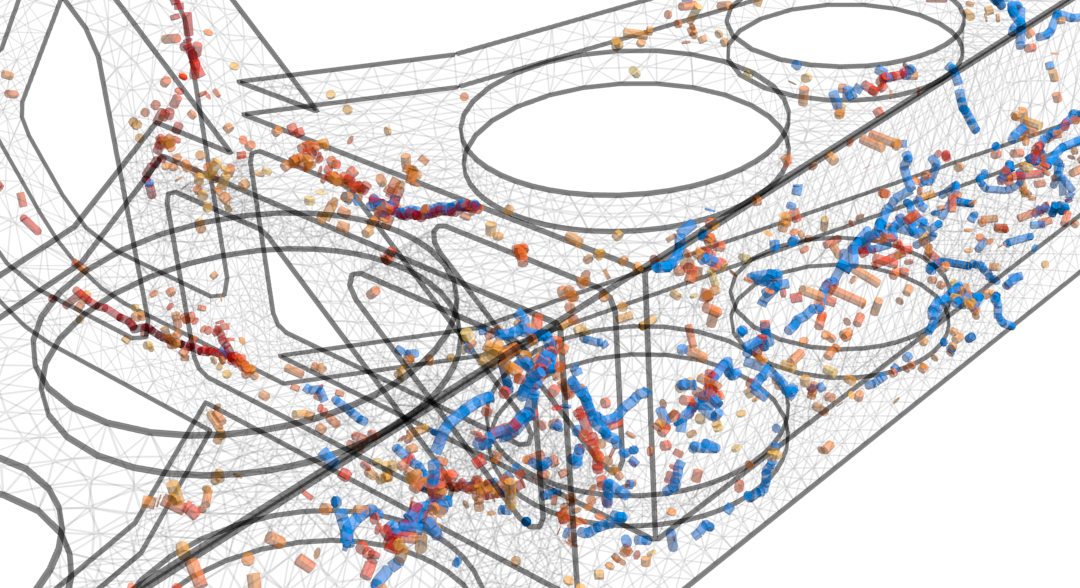
\includegraphics[width=\figurewidth]{figures/truck_bumper_topo_lines_detail2_slim}%
    };
    \begin{scope}[x={(image1.south east)},y={(image1.north west)}]
        % \draw[help lines,xstep=.1,ystep=.1] (0,0) grid (1,1);
        % \foreach \x in {0,1,...,9} { \node [anchor=north] at (\x/10,0) {\scriptsize 0.\x}; }
        % \foreach \y in {0,1,...,9} { \node [anchor=east] at (0,\y/10) {\scriptsize 0.\y}; }
        \draw[red,very thick,rounded corners] (0.3,0.57) rectangle (0.47,0.68);
    \end{scope}
    \node[label] at (image1.north west) {\textsc{Truck Bumper}};

    \node[image, below=of image1, yshift=-0.25cm] (image2)
    {
        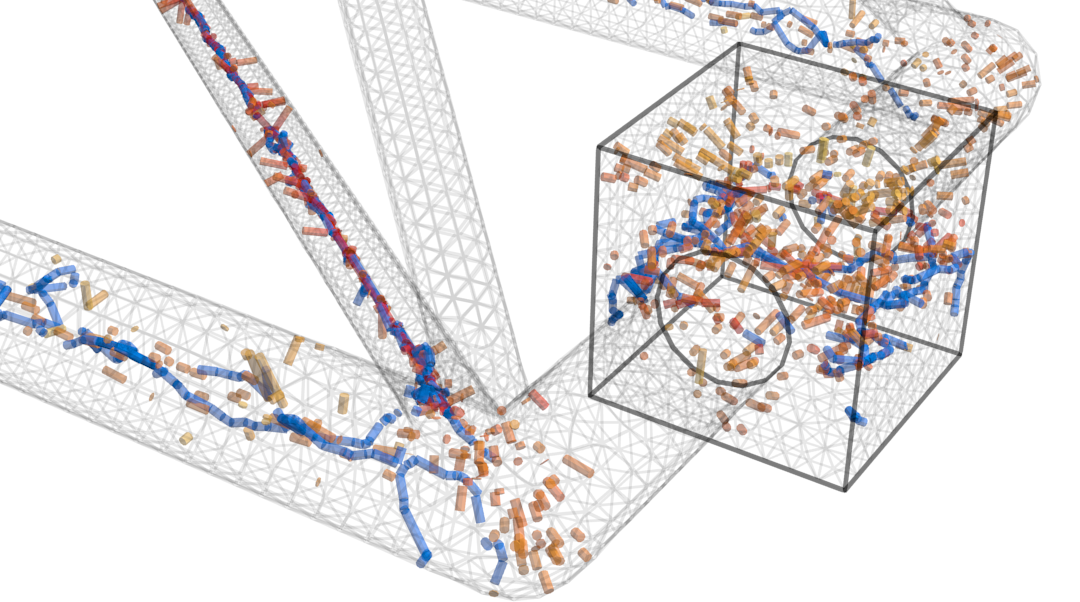
\includegraphics[width=\figurewidth]{figures/crane_topo_lines_detail1_slim}%
    };

    \node[label] at (image2.north west) {\textsc{Crane}};
\end{tikzpicture}